\lhead{Main part\hfill Study Paper, Burghard}
\clearpage
\section{Main part} \label{sec: Mainpart}
\subsection{Fundamentals: Stock Market}\label{sec: Fundamentals Stock Market}
The fundamental section gives a brief overview about the most important topics mentioned and used in the paper.
\begin{figure}[H]
	\centering
	\begin{tikzpicture}
		\path[
		mindmap,
		concept color=black,
		text=white,
		grow cyclic,
		segment length=20cm,
		level 1/.append style={level distance=5cm, sibling angle=100},
		level 2/.append style={level distance=2.5cm},
		]
		node[concept] {Fundamentals}
		[clockwise from=-40]
		child[concept color=blue] {%
			node[concept] {Stock Market}
			[clockwise from=-30]
			child {node[concept] {\nameref{sec: Stock Price}}}
			child {node[concept] {\nameref{sec: Market Faktors}}}
			child {node[concept] {\nameref{sec: Stock Selection}}}
		}
		child[concept color=violet] {%
			node[concept] {Technical}
			[clockwise from=0]
			child {node[concept] {\nameref{sec: Server}}}
			child {node[concept] {\nameref{sec: Collecting Data}}}
			child {node[concept] {\nameref{sec: Machine Learning}}}
			child {node[concept] {\nameref{sec: Storing Data}}}
		};
	\end{tikzpicture}
	\caption{Fundamentals Overview}
	\label{fig: fundamentals chart}
\end{figure}
\subsubsection{Stock Price}\label{sec: Stock Price}
The price of a stock is determined by supply and demand. If more people want to buy a stock, the price will go up. If more people want to sell a stock, the price will go down.
The question is whether people think a companies stock will rise or fall in the future. Sometimes companies perform excellent, but the stock price is falling because investors are thinking the company will fail in the future. It is important to note that stock prices can be volatile and can fluctuate wildly in the short term. However, over the long term, stock prices tend to track the underlying performance of the companies they represent. \cite{graham1934intelligent}
The difficult part is, that stock prices are not only determined by objective facts and figures, but rather the feelings of traders and buyers about the future of the company. So the project is more of an attempt to predict buyers feelings than a company's success. Or as Philip Fisher said:\\
\\
\textit{\grqq The stock market is filled with individuals who know the price of everything, but the value of nothing\grqq{}} (Philip Fisher 1907-2004)
\subsubsection{Stock Selection}\label{sec: Stock Selection}
Choosing stocks is a complex process that involves a variety of factors. There is no one-size-fits-all approach, the best way to choose stocks will vary depending on the investors individual goals and risk tolerance. However, there are some general principles that you can follow to improve your chances of success.\\
\begin{itemize}%Agenda to choose a stock
	\item \textbf{Identify a sector:}\\
	Firstly the sector needs to be identified. This can be done based on the long-term trends in each sector. 
	\item \textbf{Screen for stocks:}\\
	The next step is to screen for individual stocks. For starters can be done by looking at the biggest companies in that sector.
	\item \textbf{Review the fundamentals:}\\
	Once a list of potential stocks has been created, the next step is to review the fundamentals of each company in more detail. 
	\item \textbf{Select based on Scores:}\\
	Each share can collect points for the market factors. In each category from 0-10 points. The company with the best score in a category receives 10 points. After adding up all the points from all categories, the company with the highest total can be selected.\\
\end{itemize}
\subsubsection{Market Factors}\label{sec: Market Faktors}
There are a number of financial ratios that could influence the stock development. The most important ones are explained here.
Some factors can be drawn directly from \ac{API}s while others will be calculated. Factors 1-4 are company specific while 5-11 are about the country and the overall market situation.\\
\begin{itemize}
	\item \textbf{Market Capitalization}: The total value of a company in the stock market, calculated by multiplying the current stock price by the total number of outstanding shares.
	\begin{align}\text{Market Capitalization} = \text{Stock Price} \cdot \text{Total Outstanding Shares} \end{align}

	
	\item \textbf{Earnings}: The profits generated by a company over a specific period, typically reported quarterly or annually.
	\begin{align} \text{Earnings} = \text{Total Revenue} - \text{Total Expenses} \end{align}
			
	\item \textbf{Earnings Per Share (EPS)}: Calculated as a company's total earnings divided by its total outstanding shares, indicating profitability on a per-share basis.
	\begin{align} \text{EPS} = \frac{\text{Net Income}}{\text{Total Outstanding Shares}} \end{align}
	
	\item \textbf{Price-to-Earnings Ratio (P/E Ratio)}: Calculated by dividing a company's stock price by its earnings per share, used to assess a stock's valuation.
	\begin{align} \text{P/E Ratio} = \frac{\text{Stock Price}}{\text{EPS}} \end{align}
	
	\item \textbf{Exchange Rate}: The rate at which one currency can be exchanged for another.
	\begin{align} \text{Currency Rate} = \frac{\text{Value of Currency A}}{\text{Value of Currency B}} \end{align}
	
	\item \textbf{Retail Sales}: The total sales of goods and services by retail stores within a specific time frame, often used as an indicator of consumer spending and economic health.
	\begin{align} \text{Retail Sales} = \sum (\text{Sales of Individual Retail Stores}) \end{align}
	
	\item \textbf{\ac{CPI}}: A measure that examines the weighted average of prices of a basket of consumer goods and services, used to assess inflation's impact on the cost of living.
	\begin{align} \text{CPI} = \frac{\text{Cost of Market Basket in Current Year}}{\text{Cost of Market Basket in Base Year}} \cdot 100 \end{align}
	
	\item \textbf{Unemployment Rate}: The percentage of the total labor force that is unemployed and actively seeking employment, serving as an indicator of economic health.
	\begin{align} \text{Unemployment Rate} = \left( \frac{\text{Number of Unemployed People}}{\text{Total Labor Force}} \right) \cdot 100 \end{align}
	

	\item \textbf{Federal Funds Rate}: The interest rate at which banks lend reserves to other banks overnight, set by the Federal Reserve to influence economic growth and inflation.
	\begin{align} \text{Federal Funds Rate is set by the Federal Open Market Committee} \end{align}
	
	\clearpage
	
	\item \textbf{\ac{GDP}}: \ac{GDP} adjusted for inflation, providing a measure of a country's economic output.
	\begin{align} \text{Real GDP} = \frac{\text{Nominal GDP}}{\text{GDP Deflator}} \end{align}
	
	\item \textbf{Inflation}: The rate at which the general level of prices for goods and services is rising, eroding purchasing power.
	\begin{align} \text{Inflation Rate} = \left( \frac{\text{CPI in Current Year} - \text{CPI in Previous Year}}{\text{CPI in Previous Year}} \right) \cdot 100 \end{align}
\end{itemize}

Choosing stocks is a complex process that requires careful research and analysis. However, by following the steps outlined above, investors can increase their chances of success. \cite{CFITeam2023}

\subsection{Fundamentals: Technical}\label{sec: Fundamentals Methods}
\subsubsection{Storing Data}\label{sec: Storing Data}
\ac{CSV}, \ac{JSON}, or Databases are all data formats/ methods that are commonly used to store and exchange data. These formats are all text-based, which makes them easy to read and write and they are also supported by a wide variety of software applications.\\
\begin{itemize}
\item\textbf{\ac{CSV}} is a simple format that stores data in a table-like format. Each row in a \ac{CSV} file represents a single record, and the columns are separated by commas. \ac{CSV} files are commonly used to store and exchange tabular data, such as financial records and product catalogs.

\item\textbf{\ac{JSON}} is a lightweight data-interchange format that is easy for humans to read and write. \ac{JSON} stores data in a hierarchical object structure, which makes it ideal for storing complex data structures, such as customer information and product catalogs. \ac{JSON} is also commonly used in web development and \ac{API}s.

\item\textbf{Database} as storage method is a structured collection of data that is organized so that it can be easily accessed, managed, and updated. Databases are used to store a wide variety of data, including customer information, product catalogs, financial records, and more. Databases are made up of tables, which are collections of rows and columns. Each row represents a single record in the database, and each column represents a different attribute of that record. Common databases that can be used in Python are \ac{MySQL}. The query language for Databases is \ac{SQL}.\cite{bigdatainsiderDataNoSQL}
\end{itemize}
\subsubsection{Machine Learning}\label{sec: Machine Learning}
\ac{ML} is a subtype of \ac{AI} that allows software applications to become more accurate in predicting outcomes without being explicitly programmed to do so. \ac{ML} algorithms use historical data as input to predict new output values. There are three main types of \ac{ML}\cite{burkov2019hundred}:\\
\begin{itemize}%List of Machine Learning
	\item In \textbf{supervised learning}, the algorithm is trained on a set of labeled data, where each input has a known output. The algorithm learns to map the inputs to the outputs, and can then be used to predict the outputs of new inputs.
	\item In \textbf{unsupervised learning}, the algorithm is trained on a set of unlabeled data. The algorithm learns to find patterns and relationships in the data without being told what to look for. This can be used for tasks such as clustering data points into groups or identifying anomalies.
	\item In \textbf{reinforcement learning}, the algorithm learns to take actions in an environment in order to maximize a reward. The algorithm is given feedback on its actions, and it learns to take actions that lead to higher rewards. This can be used for tasks such as training a robot to walk or training a game-playing agent.\\
\end{itemize}
Machine learning is used in a wide variety of applications, including:\\
\begin{itemize}%List of ML Applications
	\item \textbf{Recommendation systems:} Machine learning is used to recommend products to customers, movies to viewers, and music to listeners. For example, Netflix uses machine learning to recommend movies to its users based on their viewing history.
	\item \textbf{Fraud detection:} Machine learning is used to detect fraudulent transactions and other types of fraud. For example, banks use machine learning to detect fraudulent credit card transactions.
	\item \textbf{Image recognition:} Machine learning is used to identify objects and people in images. For example, self-driving cars use machine learning to identify objects on the road, such as other vehicles and pedestrians.\\
\end{itemize}
\ac{ML} is a powerful tool that can be used to solve a wide range of problems. It is important to note that \ac{ML} algorithms are only as good as the data they are trained on. If the data is biased or incomplete, the algorithm will learn the biases and produce inaccurate results.

\subsubsection{Collecting Data}\label{sec: Collecting Data}
A set of rules and specifications that define how software components should interact with each other is referred to as \ac{API}. Different software applications can communicate with each other and exchange data via \ac{API}s. Once a \ac{API} provider has been identified, an account must be created to obtain a \ac{API} key. The key is required to make requests and retrieve data from the \ac{API}.\\
The following shows an example of an \ac{API} request:\\
\begin{lstlisting}[language=bash]
https://www.alphavantage.co/query?function=TIME_SERIES_DAILY&symbol=IBM&apikey=demo
\end{lstlisting}
The violet term called function is the most important part. It describes what type of data will be returned. In this case "TIME\_SERIES\_DAILY". Separated by "\&", other parameters are defined, like the stock symbol.\\
\\
In Python, the library called "requests" can be used to simplify \ac{API} requests.
\subsubsection{Servers}\label{sec: Server}
Servers can serve various purposes, such as hosting websites, storing files, managing emails, or running specific applications accessed by multiple users. In this case the server will be used to run the data collection program every day automatically. The following list describes three methods that can be used to make an server.\\
\begin{itemize}
	\item \textbf{Laptop}: A server can be created using a laptop by configuring scheduled tasks or "cron jobs" (if using Unix/Linux) to execute the program at specific times. The laptop should be connected to power and kept powered on at the scheduled execution times. The downside is the enormous power consumption even in standby.
	\item \textbf{Raspberry Pi}: A \ac{PI} can be utilized as a dedicated server. An operating system (like Debian 11) can be installed and with timers the program can be configured to run at specified intervals. The \ac{PI} can be left running continuously, serving as a low-power, dedicated server.	
	\item \textbf{Cloud Provider}: Services provided by cloud providers like Google Cloud, or Azure allow server instances to be deployed. A server instance can be created, necessary software can be installed, and scheduled tasks can be configured using built-in services. The program can be set up to be run on the cloud server according to scheduling requirements.\\
\end{itemize}
\clearpage
\subsection{Related Work}\label{sec: Related Work}
The following text with give an overview over the state of the art. Its chronological sorted after the publication year.\\
\\
\begin{table}[H]%Literature Overview
	\centering
	\begin{tabularx}{\textwidth}{|c|c|X|}
		\hline
		\rowcolor{lightgray}
		\hline
		\textbf{Reference} & \textbf{Year} & \textbf{Topic} \\ \hline
		\cite{mittermayer2004} & 2004 & Intraday stock price trend forecasting \\ \hline
		\cite{schumaker2009textual} & 2009 & Impact of financial news articles on stock market prediction \\ \hline
		\cite{Mittal2011StockPU} & 2010 & Stock prediction through Twitter sentiment analysis \\ \hline
		\cite{smailovic2013predictive} & 2013 & Use of Twitter feeds to forecast stock closing prices \\ \hline
		\cite{geva2014empirical} & 2014 & Assessing effectiveness of combining market and textual news data \\ \hline
		\cite{batra2018integrating} & 2018 & Sentiment analysis to predict stock price movement \\ \hline
		\cite{vignesh2018applying} & 2018 & Comparison of \ac{SVM} and \ac{LSTM} models for stock prediction \\ \hline
		\cite{ren2018forecasting} & 2018 & Leveraging user-generated content for sentiment analysis \\ \hline
		\cite{zhong2019predicting} & 2019 & Application of \ac{DNN} for stock prediction \\ \hline
		\cite{araci2019finbert} & 2019 & Addressing challenges of financial sentiment analysis \\ \hline
		\cite{ferreira2021artificial} & 2021 & Comprehensive review on AI in stock market investments \\ \hline
		\cite{Jihan2023} & 2023 & Stock price prediction using sentiment analysis and deep learning \\ \hline
	\end{tabularx}
	\caption{Literature Research Overview}
	\label{tab:literature}
\end{table}

Mittermayer (2004) investigated intraday stock price trend forecasting using text mining techniques. A prior system called "NewsCATS" employed unstructured data, a 392-keyword dictionary, and \ac{ML} algorithms to categorize press releases into "Good News", "Bad News" or "No Movers." Notably, they selectively included news articles with specific attributes, excluding press releases that lacked a ticker symbol, contained multiple ticker symbols, lacked references to the company's stock exchange, referred to non-NYSE or NASDAQ-AMEX exchanges, or had no subject code. The profit margin was around 0.11\% per trade happening 60 minutes after a press publication.\cite{mittermayer2004}\\

Schumaker and Chen (2009) explored the impact of financial news articles on stock market prediction using three textual representations: Bag of Words, Noun Phrases, and Named Entities. They assessed the ability of these representations to predict discrete stock prices twenty minutes after article release, employing a \ac{SVM} derivative, which outperformed linear regression. Notably, the Noun Phrase representation scheme proved more effective than the conventional Bag of Words. The resulted in an prediction accuracy of 50.8\%.\cite{schumaker2009textual}\\

Mittal (2010) explored stock prediction through Twitter sentiment analysis. The study applied sentiment analysis and machine learning principles to uncover the correlation between "public sentiment" and "market sentiment." Sentiment analysis was performed on publicly available Twitter data, categorizing tweets into four classes - "Calm", "Happy", "Alert", and "Kind". To optimize the analysis process, tweet filtering was applied, considering only tweets containing specific keywords related to expressing feelings ("I feel...", "I am...", "It makes me..."). The paper introduced a unique word list based on the \ac{POMS} questionnaire and employed various machine learning techniques, including the  \ac{SOFNN} for prediction, which was able to get 76\% accuracy.\cite{Mittal2011StockPU}\\

Smailović et al. (2013) investigated the use of Twitter feeds to forecast stock closing prices based on public opinion regarding companies and their products. The study involved categorizing tweets into three sentiment categories (positive, negative, and neutral) and explored the potential influence of emotions on stock market behavior. The research aimed to determine whether sentiment analysis of Twitter data could provide valuable insights into stock price movements. The conlusion was that: "[...]the stock market itself can be considered as a measure of social mood."\cite{smailovic2013predictive}\\

Geva and Zahavi (2014) conducted a study to assess the effectiveness of combining numerical market data and textual news data, utilizing data mining techniques to predict intraday stock returns. They emphasized the importance of integrating both data sources to capture joint patterns that might go unnoticed when each source is used independently. They used an new method that was not found in other papers: \textit{"Due to the instability of early-morning
	trades, we began the analysis at 9:45. We stopped making predictions
	at 15:00 each day."} The research demonstrated that a trading recommendation system incorporating both market data and news data can leverage the synergy between these two distinct information sources and potentially detect their combined influence on stock prices.\cite{geva2014empirical}\\
\\
Batra and Daudpota (2018) introduced the concept of utilizing Sentiment Analysis to predict stock price movement based on the sentiment of individuals, demonstrating its influence on stock prices. They conducted sentiment analysis on tweets related to Apple products extracted from StockTwits, a social networking site, from 2010 to 2017. The sentiment score of each tweet was calculated using \ac{SVM}, categorizing them as bullish or bearish. By combining sentiment scores with market data from Yahoo Finance, they built an \ac{SVM} model for predicting the next day's stock movement, achieving an accuracy of 76.65\% in stock prediction. This research highlighted the positive relationship between public opinion and market data.\cite{batra2018integrating}\\

Vignesh (2018) compared \ac{SVM} and \ac{LSTM} models for stock price prediction, aiming to predict whether stock prices would increase or decrease. The study's dataset spanned from 2011 to 2015, with a focus on Yahoo and Microsoft data. While the research achieved prediction accuracy for stock price rise or fall, it highlighted the limitation of not being able to predict specific price changes. \ac{SVM} yielded an accuracy of 65.2\%, and \ac{LSTM} showed a slightly improved accuracy of 66.83\%.\cite{vignesh2018applying}\\

Ren, Wu, and Liu (2018) recognized the significance of investor sentiment in the stock market and leveraged user-generated textual content from the internet for sentiment analysis. They integrated sentiment analysis with \ac{SVM} based machine learning. By considering the day-of-week effect and constructing reliable sentiment indexes, the research achieved remarkable results. The accuracy of forecasting the movement direction of the SSE 50 Index significantly improved, reaching up to 89.93\% after introducing sentiment variables, enhancing decision-making for investors. These findings suggest that sentiment analysis can be a leading indicator for stock market behavior, possibly reflecting valuable information about asset fundamental values.\cite{ren2018forecasting}\\

Zhong and Enke (2019) explored the application of \ac{DNN} and \ac{PCA} for predicting the daily return direction of the SPDR S\&P 500 \ac{ETF} based on financial and economic features. Their study revealed that \ac{DNN}s with \ac{PCA}-represented data outperformed other methods in terms of classification accuracy and trading strategy performance. The research emphasized the significance of direction forecasts in trading systems, showing their superiority over level forecasts, especially in a real-world trading environment, as successful direction forecasts are more likely to be profitable.\cite{zhong2019predicting}\\

Araci (2019) addressed the challenges of financial sentiment analysis, primarily the specialized language and limited labeled data in the financial domain. To overcome these challenges, they introduced \ac{FinBERT}, a language model based on BERT. \ac{FinBERT} demonstrated significant improvements over state-of-the-art \ac{ML} methods in financial sentiment analysis, achieving an accuracy of 97\% and surpassing \ac{LSTM}-based models.\cite{araci2019finbert}\\

Ferreira, Gandomi, and Cardoso (2021) conducted a comprehensive literature review on the application of \ac{AI} in stock market investments, analyzing a sample of 2,326 papers published between 1995 and 2019 from the Scopus website. The study provides valuable insights into the advancements and trends in this field over the years, contributing to the understanding of \ac{AI}'s role in stock market trading. The paper was used as an starting point for this papers research.\cite{ferreira2021artificial}\\

Kim, Kim, and Choi (2023) explored stock price prediction by combining mathematical-based sentiment analysis and deep learning models. They leveraged the \ac{FinBERT} Transformer Model, designed for financial language processing, along with \ac{LSTM}, to investigate the influence of human sentiment on stock movements, particularly in textual data. This specialized language model demonstrated impressive forecasting accuracy, achieving a directional accuracy of 71.18\% and a trading return of 8.50\%. The study contributes to the understanding of how transformer models like \ac{FinBERT} can play a crucial role in stock market prediction.\cite{Jihan2023}\\
\\
\textbf{Conclusion}\\
In the realm of stock market prediction, sentiment analysis stands out as a vital tool, utilizing textual data to gauge investor sentiment. \ac{ML} models, including \ac{SVM}, \ac{LSTM}, and transformer models such as  \ac{FinBERT}, have demonstrated their effectiveness in enhancing prediction accuracy. Reliable data sources like Yahoo Finance and The New York Times have played a significant role in model training and evaluation.\\
\\
Building on the best proven algorithms the program will use \ac{FinBERT} to analyze sentiment in news because the method has the highest accuracy. Most of the papers used either sentiment analysis or technical factors. To get the best out of both methods the program will use each information source. Furthermore, \ac{LSTM} seems to be the best method to predict stock prices, so the implementation starts with this method.
\clearpage
\subsection{Concept Phase}\label{sec: Concept Phase}
The overall plan can be summarized as follows: First, select a promising stock based on the criteria and formulas. Next, gather data about the stock through \ac{API}s and train an \ac{AI} model on the collected data using machine learning techniques Subsequently, collect live data and perform analysis to predict stock development. To begin, a specification sheet is created to set our initial direction. Following that, a morphological box will assist in selecting among various options.
\subsubsection{Specification Sheet}\label{sec: Specification Sheet}
Some of the requirements are functional and some are non-functional (optional). The following list describes the functional points the final program needs to be able to do.
\paragraph{Essential Requirements:}
\begin{enumerate}
	\item Recommend the user to buy sell or hold a specific stock
	\item Collect training data daily
	\item Predict short, middle and long term stock development
	\item Outperform the "hold strategy" for 1\% long term (minimum 1 year)
\end{enumerate}

\paragraph{Optional requirements:}

\begin{enumerate}
	\item Machine learning model is optimized for speed and efficiency
	\item Robust security measures to safeguard training data
	\item Encryption is used for data transmission and storage
	\item Simulate stock investments with virtual portfolios
	\item User interface for inputting chosen stocks and viewing predictions and insights
	\item System is designed to handle a growing user base and increasing data volume
	\item Compliance with relevant financial regulations and data privacy laws
	\item Document the system architecture, data sources, and algorithms for internal reference
\end{enumerate}


\clearpage
\subsubsection{Timeline}\label{Timeline}
The milestones and dates that are targeted are listet in the table below.

\begin{table}[H]
	\centering
	\renewcommand\arraystretch{1.4}
	\begin{tabular}{@{\,}r <{\hskip 2pt} !{\foo} >{\raggedright\arraybackslash}p{5cm}}
		\toprule
		\addlinespace[1.5ex]
		04.10.2023 & Project starts\\
		06.10.2023 & Project registered\\
		08.10.2023 & Paper is set up and formated\\
		13.10.2023 & Advisor Steffen Quadt is assigned\\
		20.10.2023 & List of Requirements finished\\
		22.10.2023 & Overall Projectmanagement and planning finished\\
		23.10.2023 & TESTAT 1 is uploaded to Moodle\\
		04.11.2023 & Research related Work is done\\
		05.11.2023 & All Variations of morphological box are decided\\
		05.11.2023 & Stock is chosen --> Adobe\\
		07.11.2023 & TESTAT 2 is uploaded to Moodle\\
		12.11.2023 & \ac{API} program is finished and can collect data\\
		18.11.2023 & The program runs automatically on a server every day\\	
		22.12.2023 & Project Part 1 ends\\
		25.03.2024 & Project Part 2 starts...\
	\end{tabular}
	\captionof{table}{Timeline}
	\label{tab: timeline}
\end{table}
\clearpage
\subsubsection{Morphological Box}\label{sec: Morphological Box}
\begin{table}[H]
	\centering
	\begin{tabular}{c}
		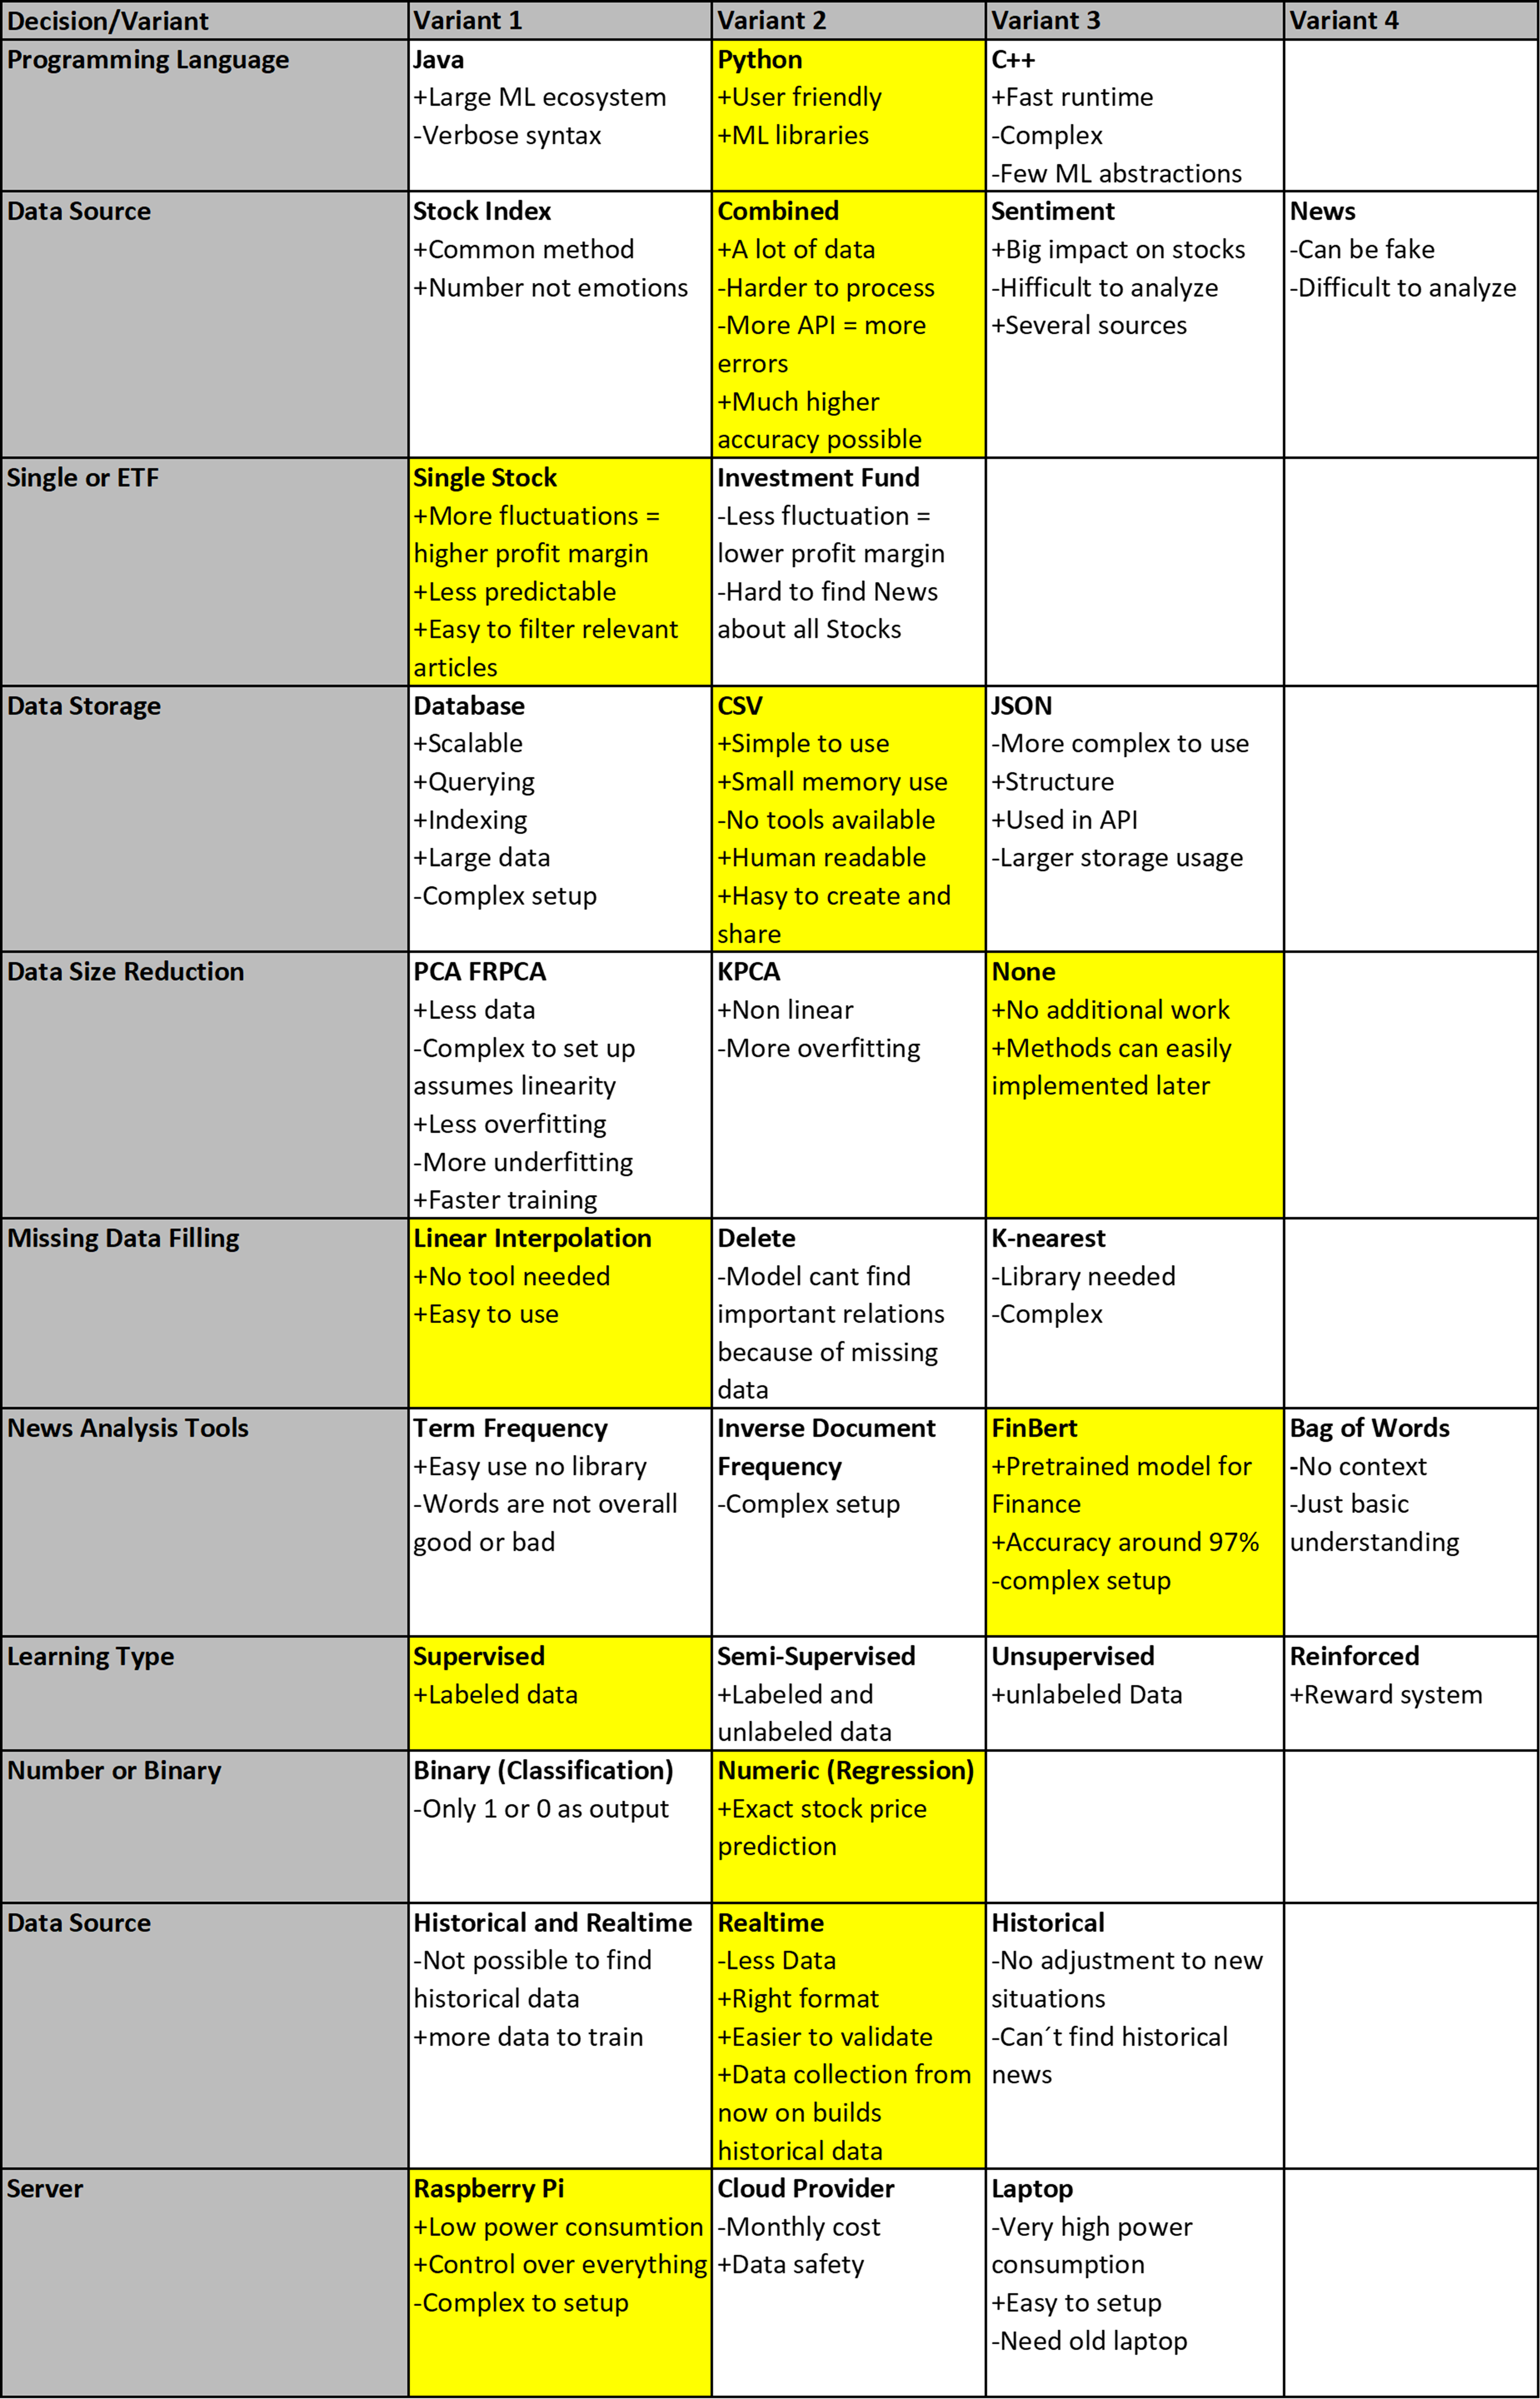
\includegraphics[width=0.9\textwidth]{mainpart/img/morphbox.png} \\
	\end{tabular}
	\caption{Morphological Box}
	\label{tab: morphological box}
\end{table}
The selected variants, indicated by the cells highlighted in yellow, are based on a thorough evaluation of scientific work and a consideration of their respective advantages and disadvantages. These decisions are made after considering what can best be implemented and what is most suitable for the project. 
\subsection{Implementation}\label{sec: Implementation}
The following sections will use the fundamentals and the methods chosen to implement the program. First the stock will be chosen. Afterwards the \ac{API}-Provider needs to be chosen. Then the program to collect the data will be written. When finished everything needs to be put on a server to run automatically daily. The last step is to prevent failures and data loss.
\subsubsection{Select Stock}\label{sec: Choose promising Stock}
The first version of the program will only be able to analyze one specific stock. The right company to invest in is as important as the right program.
Firstly the market sector is selected:\\
\\
\textbf{10 biggest Market Sectors:}
\begin{enumerate}
	\item Healthcare
	\item Financial Services
	\item Technology
	\item Consumer Discretionary
	\item Energy
	\item Industrial
	\item Materials
	\item Consumer Staples
	\item Utilities
	\item Real Estate\\
\end{enumerate}

The technology sector is an ideal choice for equity investment as it is home to some of the world's largest companies, all of which operate predominantly in the technology sector, guaranteeing significant growth prospects and innovative advances.\\
\\
\textbf{Top 3 Stocks from Technology Sector}\\
The first selection of the top 3 stocks from the technology sector was made on October 12, 2023 at 9 p.m. with the help of "Yahoo Finance" (\url{finance.yahoo.com}). The website offers search filters for various parameters. The aim of the program, which is developed here, is to predict the long-term development of shares so that a stable share without major fluctuations and yet with high growth opportunities is searched for. Therefore the selected categories and parameters were:\\
\begin{itemize}
	\item Sector: Technology
	\item Market Capitalization: Mega Cap
	\item Sort by: Previous year growth\\
\end{itemize}
Stocks with no available information were excluded, as were stocks with a currency other than \ac{USD} or \ac{EUR}.\\
\\
\textbf{Compare top 3 Stocks}\\
Price, market capitalization, \ac{P/E ratio}, and \ac{EPS} data were sourced from Yahoo Finance. Yearly growth data was obtained from the Google Stocks Overview (\url{google.com/finance}). "Revenue Growth" information was provided by Makrotrends (\url{macrotrends.net}). Oracle information was provided in USD and was converted to EUR at the current exchange rate of 0.95 \ac{EUR} per \ac{USD}. Additionally, the Danelfin \ac{AI} was employed to assign a 1-10 score to each stock, which can be accessed (\url{danelfin.com}).\\
\\
Each parameter is normalized to a scale of 1-10 (light brown lines), where the highest score is always 10. The final score for each stock is the sum of these 1-10 ratings. The table is displayed below:
\begin{table}[H]
	\centering
	\begin{tabular}{c}
		\includegraphics[width=\textwidth]{mainpart/img/stocks.png} \\
	\end{tabular}
	\caption{Choosing Stock Calculation Sheet}
	\label{tab: stocks}
\end{table}
Adobe, with the highest score sum, is the chosen option. Below is a chart displaying its performance over the past year. The vertical axis displays the stock price in \ac{EUR} and the horizontal axis represents the time.
\begin{figure}[H]
	\centering
	\begin{tikzpicture}
		\node [anchor=south west] (image) at (0,0) {\includegraphics[width=1\textwidth,keepaspectratio]{"Mainpart/img/adobe_chart.png"}};
		\begin{scope}[
			x={($0.1*(image.south east)$)},
			y={($0.1*(image.north west)$)}]
		\end{scope} 
		%Rahmen um Bild
		\draw(current bounding box.north west) rectangle (current bounding box.south east);
	\end{tikzpicture}
	\caption[Adobe Chart]{Adobe Chart (\url{google.com/finance}, accessed: 13.10.2023)}
	\label{fig: Adobe Chart Last Year}
\end{figure}
\subsubsection{API Provider}\label{sec: api provider}
Alpha Vantage was chosen for the stock market prediction project primarily due to its diverse and comprehensive financial data offerings. Despite the limit of 25 free daily requests, an large amount of data is provided for the project's needs including: real-time data, technical indicators, and fundamental data. The platform's ease of integration and clear documentation were crucial factors in the choice, enabling quick access and utilization of the data within predictive models.\\
\\
The importance of access to various news sources for complete information was decisive for the choice of \url{newsapi.org}. Recognizing the significance of gathering news from varied outlets, the platform offers a wide spectrum of sources, enabling access to multiple perspectives and diverse content. This variety of sources increases the depth and range of information available for analysis and insight. The site gives unlimited free queries from one month in the past to now.\\
\\
The following tables shows all the \ac{API}s, the provider and the data size. The total folder size from one day of collecting data is around 1.3 \ac{MB}.
\begin{table}[H]
	\centering
	\begin{tabular}{c}
		\includegraphics[width=\textwidth]{mainpart/img/api.png} \\
	\end{tabular}
	\caption{\ac{API} Overview}
	\label{tab: API}
\end{table}
\subsubsection{Write Code to Collect Data}\label{sec: dc code}
The Python script utilizes several libraries, including "requests", "json", "datetime", "re", and "os", along with custom configurations from an extra file. The primary function of this script is to gather financial data and news from various \ac{API}s, storing the obtained \ac{JSON} responses in files organized by date.\\
\\
The script begins by printing essential information for user reference, such as the date of data collection, stock details, and other relevant parameters as seen in \autoref{fig: dc out}.
\begin{figure}[H]
	\centering
	\begin{tikzpicture}
		\node [anchor=south west] (image) at (0,0) {\includegraphics[width=0.5\textwidth,keepaspectratio]{"Mainpart/img/dc_out.png"}};
		\begin{scope}[
			x={($0.1*(image.south east)$)},
			y={($0.1*(image.north west)$)}]
		\end{scope} 
		%Rahmen um Bild
		\draw(current bounding box.north west) rectangle (current bounding box.south east);
	\end{tikzpicture}
	\caption{Data Collector Program Output 1}
	\label{fig: dc out}
\end{figure}
It sets up a directory structure and prepares a list of URLs pointing to different \ac{API}s providing financial data and news related to the stock and market. The \ac{API}-Keys and other Parameters the program needs are stored separately in a configuration file so they can be changed without editing the source code.\\
\\
Following this, the script iterates through each URL, initiating API requests via "requests.get()" and handles the corresponding \ac{JSON} responses. 
\begin{figure}[H]
	\centering
	\begin{tikzpicture}
		\node [anchor=south west] (image) at (0,0) {\includegraphics[width=0.5\textwidth,keepaspectratio]{"Mainpart/img/dc_out_2.png"}};
		\begin{scope}[
			x={($0.1*(image.south east)$)},
			y={($0.1*(image.north west)$)}]
		\end{scope} 
		%Rahmen um Bild
		\draw(current bounding box.north west) rectangle (current bounding box.south east);
	\end{tikzpicture}
	\caption{Data Collector Program Output 2}
	\label{fig: dc out2}
\end{figure}
Each day's data is organized into folders named according to the YYYYMMDD syntax, signifying the precise date of data collection. This structuring method optimally maintains data organization and facilitates seamless sorting based on date, ensuring consistent chronological arrangement even after potential modifications or updates.\\
\\
The significance of displaying the output in the console lies in providing users with real-time feedback about the script's progress, ensuring visibility into the data collection process, and offering insights into any encountered errors or limitations due to \ac{API} constraints. This transparency helps users monitor the execution and status of the data collection procedure, facilitating informed decision-making and troubleshooting if necessary.
\subsubsection{Server setup}\label{sec: server setup}
The server setup for daily automated execution of the Python script was initiated using a \ac{Pi}, chosen for its low power consumption. An bundle with all the needed parts including heat sinks and cables is used.
\begin{figure}[H]
	\centering
	\begin{tikzpicture}
		\node [anchor=south west] (image) at (0,0) {\includegraphics[width=0.8\textwidth,keepaspectratio]{"Mainpart/img/raspi.png"}};
		\begin{scope}[
			x={($0.1*(image.south east)$)},
			y={($0.1*(image.north west)$)}]
		\end{scope} 
		%Rahmen um Bild
		\draw(current bounding box.north west) rectangle (current bounding box.south east);
	\end{tikzpicture}
	\caption[Raspberry Pi 4 Bundle]{Raspberry Pi 4 Bundle (\url{reichelt.de}, accessed: 26.11.2023)}
	\label{fig: Raspi}
\end{figure}
The \ac{Pi} is connected to an external 1 TB \ac{SSD}. Debian was installed on the \ac{Pi}, providing a stable operating system suited for the device's architecture. The code was transferred to the device, preparing it for scheduled execution. A ".timer" and ".service" file were created to enable systematic scheduling via systemd.\\
\\
The coordination of the data collection program was facilitated by the ".service" file. Upon activation, the service initiated the Python script, enabling the execution of numerous \ac{API} requests and the meticulous collection and storage of data on the local drive of the \ac{Pi}. 
\subsubsection{Redundancy and Checkup}\label{sec: redundancy}
After developing the initial program, several measures were implemented to enhance its robustness and data safety. To address potential \ac{API} errors, an error handling mechanism was integrated into the program, ensuring graceful handling of any encountered errors during \ac{API} requests. Additionally, the program was augmented to retrieve and display the cumulative file size of the day's data, providing a comprehensive overview of the data collected.\\
\\
Recognizing the significance of data redundancy, an auxiliary program was designed to copy all the collected data to an external \ac{SSD}, mounted to the \ac{Pi}. Leveraging a the "shutil" libary, this program verified existing data on the \ac{SSD} and performed a complete data tree copy, effectively establishing redundancy for all collected information.\\
\\
Furthermore, to maintain a transparent and informative process, an email notification system was established. The data collection program gives information about the \ac{API} requests and the data size and writes it into an .txt file, the backup program confirms the backup and adds the information to the same text file. A Python script utilizes the "EmailMessage" module to compose an email. It reads the content from the text file mentioned before and sets up an email message, defining sender, recipient, subject, and content. Using \ac{SMTP} and \ac{SSL} from "smtplib" libary, it establishes a secure connection with Gmail's \Ac{SMTP} server over port 465, logs in using the sender's email credentials, and sends the email to the specified recipient.\\
\begin{figure}[H]
	\centering
	\begin{tikzpicture}
		\node [anchor=south west] (image) at (0,0) {\includegraphics[width=0.5\textwidth,keepaspectratio]{"Mainpart/img/mail.png"}};
		\begin{scope}[
			x={($0.1*(image.south east)$)},
			y={($0.1*(image.north west)$)}]
		\end{scope} 
		%Rahmen um Bild
		\draw(current bounding box.north west) rectangle (current bounding box.south east);
	\end{tikzpicture}
	\caption{Example Server Mail}
	\label{fig: mails sent}
\end{figure}
To run all the programs one after another in the right order a main file is made, that starts the program inside of a \ac{venv}.
\subsubsection{Overall Program Plan}\label{sec: program plan}
The table shows all the programs and files implemented on the server to collect and save the data properly.
\begin{table}[H]
	\centering
	\begin{tabular}{c}
		\includegraphics[width=\textwidth]{mainpart/img/programs.png} \\
	\end{tabular}
	\caption{Program order, Dependencies and Descriptions}
	\label{tab: programs}
\end{table}
The timer is run at 11:11 p.m. and runs the service file. This file starts the main program that runs one script after another inside the \ac{venv}. When data collection is finished a mail is sent as seen in \autoref{fig: mails sent}.